\documentclass[a4paper,11pt]{article} % fonte 11 points, papier a4

\usepackage[french,english]{babel}   
\usepackage[T1]{fontenc}        
\usepackage{url}                
\usepackage[latin1]{inputenc}
\usepackage{lmodern}
\usepackage{setspace}
\usepackage{textcomp}
\usepackage{amsfonts}
\usepackage[table,usenames,dvipsnames]{xcolor}
\usepackage{graphicx}
\usepackage{multirow}
\usepackage{tikz}
\usepackage{fancybox}
\usepackage{colortbl}
\usepackage[final]{pdfpages}
\usepackage{multicol}
\usepackage{enumitem}
\usepackage{ifthen}
\include{colors}
\usepackage[backend=biber,style=ieee,sorting=ynt,defernumbers=true]{biblatex}
\addbibresource{listPubli.bib}
\usepackage[final]{pdfpages}
\usepackage{csquotes}

\usepackage[nomessages]{fp}

\newcommand{\myname}{\textbf{M. L\'eonardon}}

\usepackage{hyperref}
\hypersetup{colorlinks,citecolor=Paired-1, filecolor=Paired-1,linkcolor=black,urlcolor=Paired-1}

% La page
%#########
\usepackage{titlesec}
\usepackage{vmargin}            % redefinir les marges
\setmarginsrb{2cm}{2cm}{2cm}{1cm}{0cm}{0cm}{0cm}{1cm}
    
% Marge gauche, haute, droite, basse; espace entre la marge et le texte ?
% gauche, en  haut, ? droite, en bas

% Je redefinis le comportement des guillemets
%#############################################
\catcode`\?=\active
\catcode`\?=\active
\def?{\og\ignorespaces}
\def?{{\fg}}

% Diverses nouvelles commandes
%#############################

%%Cleardoublepage
\makeatletter
\renewcommand{\cleardoublepage}{
\clearpage\thispagestyle{empty}
\if@twoside
\ifodd\c@page
\else
\hbox{}\newpage
\fi
\fi
}
\makeatother

% Pour laisser de l'espace entre les lignes du tableau
\newcommand\espace{\vrule height 20pt width 0pt}
\newcommand{\HRule}[2]{{\centering\rule{#1}{#2}}}

\definecolor{lightlightblue}{rgb}{0.75,0.85,1}
\definecolor{lightlightgray}{rgb}{0.93,0.93,0.93}
\definecolor{lightlightgray2}{rgb}{0.8,0.8,0.8}
\definecolor{lightlightlightgray}{rgb}{0.98,0.98,0.98}


\setlength{\arrayrulewidth}{0.4pt}

\setcounter{tocdepth}{2}

\titleformat{\subsection}[block]{}{}{1em}
{
    \vspace{-1.3cm}
    \begin{flushleft}
    \begin{minipage}{\linewidth}
    \HRule{\linewidth}{0.2mm}\\[5pt]
    \centering
    \bf \thesubsection\quad
}
[
    \HRule{\linewidth}{0.2mm}
    \end{minipage}
    \end{flushleft}
]

\titleformat{\section}[block]{\Large \sc}{\thesection}{1em}{\centering}

\newcommand{\tabcv}[2]{
\begin{minipage}[t]{0.12\linewidth}
\textbf{\footnotesize #1}
\end{minipage}\hfill
\begin{minipage}[t]{0.85\linewidth}
#2
\end{minipage}
\vspace{1em}
}

\renewcommand{\tabcolsep}{0.1cm}
\renewcommand{\arraystretch}{1}

\definecolor{color0}{rgb}{0,0,0}% black
\definecolor{color1}{rgb}{0.22,0.45,0.70}% light blue
\definecolor{color2}{rgb}{0.45,0.45,0.45}% dark grey

\newcommand*{\namefont}{\fontsize{28}{30}\mdseries\upshape}
\newcommand*{\titlefont}{\LARGE\mdseries\slshape}
\newcommand*{\addressfont}{\small\mdseries\slshape}
\newcommand*{\quotefont}{\large\slshape}

\newcommand*{\namestyle}[1]{{\namefont\textcolor{color0}{#1}}}
\newcommand*{\titlestyle}[1]{{\titlefont\textcolor{color2}{#1}}}
\newcommand*{\addressstyle}[1]{{\addressfont\textcolor{color2}{#1}}}
\newcommand*{\quotestyle}[1]{{\quotefont\textcolor{color1}{#1}}}


\def\version{grenoble_inp}

%###################

\titleformat{\subsection}[block]{}{}{1em}
{
    \vspace{-1.3cm}
    \begin{flushleft}
    \begin{minipage}{\linewidth}
    \HRule{\linewidth}{0.2mm}\\[5pt]
    \centering
\ifthenelse{\equal{\version}{cv_version}}
{
    \bf
}
{
    \bf \thesubsection\quad   
}
}
[
    \HRule{\linewidth}{0.2mm}
    \end{minipage}
    \end{flushleft}
]
\ifthenelse{\equal{\version}{cv_version}}
{
    \titleformat{\section}[block]{\Large \sc}{}{0em}{\centering}
}
{
    \titleformat{\section}[block]{\Large \sc}{\thesection}{1em}{\centering}
}
\ifthenelse{\equal{\version}{cv_version}}
{
    \titleformat{\subsubsection}{\bf}{}{0em}{$\bullet$\quad}   
}
{}

\begin{document}

\ifthenelse{\equal{\version}{cv_version}}
{}
{
\begin{center}\large
    %%%%%%%%%%%% Titre
    \begin{minipage}{0.95\linewidth}\centering
        \HRule{\linewidth}{0.5mm}\\
        \vspace{0.5em}
        \bf
        \LARGE{Candidature au poste de Ma�tre de Conf�rences}\\         
        \vspace{0.5em}
        \ifthenelse{\equal{\version}{grenoble_inp}}{
        \LARGE{INP de Grenoble - Poste n�4087\\}
        }{}

        \ifthenelse{\equal{\version}{lyon_insa}}{
        \LARGE{INSA Lyon - Poste n�4236\\}
        }{}

        \ifthenelse{\equal{\version}{nantes_centrale}}{
        \LARGE{Centrale Nantes - Poste n�4051\\}
        }{}

        \ifthenelse{\equal{\version}{toulouse_inp}}{
        \LARGE{INP de Toulouse - Poste n�4124\\}
        }{}

        \ifthenelse{\equal{\version}{toulouse_insa}}{
        \LARGE{INSA Toulouse - Poste n�4076\\}
        }{}
        \HRule{\linewidth}{0.5mm}
    \end{minipage}
    %%%%%%%%%%%%
    
    \vspace{1.5cm}

    \LARGE{\textbf{Candidat}}\\
    \LARGE{\textsc{Mathieu L�onardon}}\\
    \vspace{0.5cm}
    \LARGE{\textit{Qualifi� en sections 27, 61 et 63}}
    \vspace{1.5cm}

\end{center}

\renewcommand{\contentsname}{Sommaire}
\tableofcontents

\newpage
}

\ifthenelse{\equal{\version}{grenoble_inp}}{
    \includepdf[pages=1 , pagecommand={\section{D\'eclaration de candidature Galaxie}},width=\paperwidth, offset=80 -100]{candidatures/grenoble_inp}
    \includepdf[pages=2-,width=\paperwidth, offset=80 -100]{candidatures/grenoble_inp}
}{}
\ifthenelse{\equal{\version}{lyon_insa}}{
    \includepdf[pages=1 , pagecommand={\section{D\'eclaration de candidature Galaxie}},width=\paperwidth, offset=80 -100]{candidatures/lyon_insa}
    \includepdf[pages=2-,width=\paperwidth, offset=80 -100]{candidatures/lyon_insa}
}{}
\ifthenelse{\equal{\version}{nantes_centrale}}{
    \includepdf[pages=1 , pagecommand={\section{D\'eclaration de candidature Galaxie}},width=\paperwidth, offset=80 -100]{candidatures/nantes_centrale}
    \includepdf[pages=2-,width=\paperwidth, offset=80 -100]{candidatures/nantes_centrale}
}{}
\ifthenelse{\equal{\version}{toulouse_inp}}{
    \includepdf[pages=1 , pagecommand={\section{D\'eclaration de candidature Galaxie}},width=\paperwidth, offset=80 -100]{candidatures/toulouse_inp}
    \includepdf[pages=2-,width=\paperwidth, offset=80 -100]{candidatures/toulouse_inp}
}{}
\ifthenelse{\equal{\version}{toulouse_insa}}{
    \includepdf[pages=1 , pagecommand={\section{D\'eclaration de candidature Galaxie}},width=\paperwidth, offset=80 -100]{candidatures/toulouse_insa}
    \includepdf[pages=2-,width=\paperwidth, offset=80 -100]{candidatures/toulouse_insa}
}{}

\newpage


\renewcommand{\tabcolsep}{0.1cm}
\renewcommand{\arraystretch}{1}

\definecolor{color0}{rgb}{0,0,0}% black
\definecolor{color1}{rgb}{0.22,0.45,0.70}% light blue
\definecolor{color2}{rgb}{0.45,0.45,0.45}% dark grey

\section{Curriculum Vitae d�taill�}
\documentclass[a4paper,11pt]{article} % fonte 11 points, papier a4

\usepackage[french,english]{babel}   
\usepackage[T1]{fontenc}        
\usepackage{url}                
\usepackage[latin1]{inputenc}
\usepackage{lmodern}
\usepackage{setspace}
\usepackage{textcomp}
\usepackage{amsfonts}
\usepackage[table,usenames,dvipsnames]{xcolor}
\usepackage{graphicx}
\usepackage{multirow}
\usepackage{tikz}
\usepackage{fancybox}
\usepackage{colortbl}
\usepackage[final]{pdfpages}
\usepackage{multicol}
\usepackage{enumitem}
\usepackage{ifthen}
\include{colors}
\usepackage[backend=biber,style=ieee,sorting=ynt,defernumbers=true]{biblatex}
\addbibresource{listPubli.bib}
\usepackage[final]{pdfpages}
\usepackage{csquotes}

\usepackage[nomessages]{fp}

\newcommand{\myname}{\textbf{M. L\'eonardon}}

\usepackage{hyperref}
\hypersetup{colorlinks,citecolor=Paired-1, filecolor=Paired-1,linkcolor=black,urlcolor=Paired-1}

% La page
%#########
\usepackage{titlesec}
\usepackage{vmargin}            % redefinir les marges
\setmarginsrb{2cm}{2cm}{2cm}{1cm}{0cm}{0cm}{0cm}{1cm}
    
% Marge gauche, haute, droite, basse; espace entre la marge et le texte ?
% gauche, en  haut, ? droite, en bas

% Je redefinis le comportement des guillemets
%#############################################
\catcode`\?=\active
\catcode`\?=\active
\def?{\og\ignorespaces}
\def?{{\fg}}

% Diverses nouvelles commandes
%#############################

%%Cleardoublepage
\makeatletter
\renewcommand{\cleardoublepage}{
\clearpage\thispagestyle{empty}
\if@twoside
\ifodd\c@page
\else
\hbox{}\newpage
\fi
\fi
}
\makeatother

% Pour laisser de l'espace entre les lignes du tableau
\newcommand\espace{\vrule height 20pt width 0pt}
\newcommand{\HRule}[2]{{\centering\rule{#1}{#2}}}

\definecolor{lightlightblue}{rgb}{0.75,0.85,1}
\definecolor{lightlightgray}{rgb}{0.93,0.93,0.93}
\definecolor{lightlightgray2}{rgb}{0.8,0.8,0.8}
\definecolor{lightlightlightgray}{rgb}{0.98,0.98,0.98}


\setlength{\arrayrulewidth}{0.4pt}

\setcounter{tocdepth}{2}

\titleformat{\subsection}[block]{}{}{1em}
{
    \vspace{-1.3cm}
    \begin{flushleft}
    \begin{minipage}{\linewidth}
    \HRule{\linewidth}{0.2mm}\\[5pt]
    \centering
    \bf \thesubsection\quad
}
[
    \HRule{\linewidth}{0.2mm}
    \end{minipage}
    \end{flushleft}
]

\titleformat{\section}[block]{\Large \sc}{\thesection}{1em}{\centering}

\newcommand{\tabcv}[2]{
\begin{minipage}[t]{0.12\linewidth}
\textbf{\footnotesize #1}
\end{minipage}\hfill
\begin{minipage}[t]{0.85\linewidth}
#2
\end{minipage}
\vspace{1em}
}

\renewcommand{\tabcolsep}{0.1cm}
\renewcommand{\arraystretch}{1}

\definecolor{color0}{rgb}{0,0,0}% black
\definecolor{color1}{rgb}{0.22,0.45,0.70}% light blue
\definecolor{color2}{rgb}{0.45,0.45,0.45}% dark grey

\newcommand*{\namefont}{\fontsize{28}{30}\mdseries\upshape}
\newcommand*{\titlefont}{\LARGE\mdseries\slshape}
\newcommand*{\addressfont}{\small\mdseries\slshape}
\newcommand*{\quotefont}{\large\slshape}

\newcommand*{\namestyle}[1]{{\namefont\textcolor{color0}{#1}}}
\newcommand*{\titlestyle}[1]{{\titlefont\textcolor{color2}{#1}}}
\newcommand*{\addressstyle}[1]{{\addressfont\textcolor{color2}{#1}}}
\newcommand*{\quotestyle}[1]{{\quotefont\textcolor{color1}{#1}}}


\def\version{cv_version}

%###################

\titleformat{\subsection}[block]{}{}{1em}
{
    \vspace{-1.3cm}
    \begin{flushleft}
    \begin{minipage}{\linewidth}
    \HRule{\linewidth}{0.2mm}\\[5pt]
    \centering
    \bf
}
[
    \HRule{\linewidth}{0.2mm}
    \end{minipage}
    \end{flushleft}
]
\titleformat{\section}[block]{\Large \sc}{}{0em}{\centering}
\titleformat{\subsubsection}{\bf}{}{0em}{$\bullet$\quad}

\begin{document}

\renewcommand{\tabcolsep}{0.1cm}
\renewcommand{\arraystretch}{1}

\definecolor{color0}{rgb}{0,0,0}% black
\definecolor{color1}{rgb}{0.22,0.45,0.70}% light blue
\definecolor{color2}{rgb}{0.45,0.45,0.45}% dark grey

\documentclass[a4paper,11pt]{article} % fonte 11 points, papier a4

\usepackage[french,english]{babel}   
\usepackage[T1]{fontenc}        
\usepackage{url}                
\usepackage[latin1]{inputenc}
\usepackage{lmodern}
\usepackage{setspace}
\usepackage{textcomp}
\usepackage{amsfonts}
\usepackage[table,usenames,dvipsnames]{xcolor}
\usepackage{graphicx}
\usepackage{multirow}
\usepackage{tikz}
\usepackage{fancybox}
\usepackage{colortbl}
\usepackage[final]{pdfpages}
\usepackage{multicol}
\usepackage{enumitem}
\usepackage{ifthen}
\include{colors}
\usepackage[backend=biber,style=ieee,sorting=ynt,defernumbers=true]{biblatex}
\addbibresource{listPubli.bib}
\usepackage[final]{pdfpages}
\usepackage{csquotes}

\usepackage[nomessages]{fp}

\newcommand{\myname}{\textbf{M. L\'eonardon}}

\usepackage{hyperref}
\hypersetup{colorlinks,citecolor=Paired-1, filecolor=Paired-1,linkcolor=black,urlcolor=Paired-1}

% La page
%#########
\usepackage{titlesec}
\usepackage{vmargin}            % redefinir les marges
\setmarginsrb{2cm}{2cm}{2cm}{1cm}{0cm}{0cm}{0cm}{1cm}
    
% Marge gauche, haute, droite, basse; espace entre la marge et le texte ?
% gauche, en  haut, ? droite, en bas

% Je redefinis le comportement des guillemets
%#############################################
\catcode`\?=\active
\catcode`\?=\active
\def?{\og\ignorespaces}
\def?{{\fg}}

% Diverses nouvelles commandes
%#############################

%%Cleardoublepage
\makeatletter
\renewcommand{\cleardoublepage}{
\clearpage\thispagestyle{empty}
\if@twoside
\ifodd\c@page
\else
\hbox{}\newpage
\fi
\fi
}
\makeatother

% Pour laisser de l'espace entre les lignes du tableau
\newcommand\espace{\vrule height 20pt width 0pt}
\newcommand{\HRule}[2]{{\centering\rule{#1}{#2}}}

\definecolor{lightlightblue}{rgb}{0.75,0.85,1}
\definecolor{lightlightgray}{rgb}{0.93,0.93,0.93}
\definecolor{lightlightgray2}{rgb}{0.8,0.8,0.8}
\definecolor{lightlightlightgray}{rgb}{0.98,0.98,0.98}


\setlength{\arrayrulewidth}{0.4pt}

\setcounter{tocdepth}{2}

\titleformat{\subsection}[block]{}{}{1em}
{
    \vspace{-1.3cm}
    \begin{flushleft}
    \begin{minipage}{\linewidth}
    \HRule{\linewidth}{0.2mm}\\[5pt]
    \centering
    \bf \thesubsection\quad
}
[
    \HRule{\linewidth}{0.2mm}
    \end{minipage}
    \end{flushleft}
]

\titleformat{\section}[block]{\Large \sc}{\thesection}{1em}{\centering}

\newcommand{\tabcv}[2]{
\begin{minipage}[t]{0.12\linewidth}
\textbf{\footnotesize #1}
\end{minipage}\hfill
\begin{minipage}[t]{0.85\linewidth}
#2
\end{minipage}
\vspace{1em}
}

\renewcommand{\tabcolsep}{0.1cm}
\renewcommand{\arraystretch}{1}

\definecolor{color0}{rgb}{0,0,0}% black
\definecolor{color1}{rgb}{0.22,0.45,0.70}% light blue
\definecolor{color2}{rgb}{0.45,0.45,0.45}% dark grey

\newcommand*{\namefont}{\fontsize{28}{30}\mdseries\upshape}
\newcommand*{\titlefont}{\LARGE\mdseries\slshape}
\newcommand*{\addressfont}{\small\mdseries\slshape}
\newcommand*{\quotefont}{\large\slshape}

\newcommand*{\namestyle}[1]{{\namefont\textcolor{color0}{#1}}}
\newcommand*{\titlestyle}[1]{{\titlefont\textcolor{color2}{#1}}}
\newcommand*{\addressstyle}[1]{{\addressfont\textcolor{color2}{#1}}}
\newcommand*{\quotestyle}[1]{{\quotefont\textcolor{color1}{#1}}}


\def\version{cv_version}

%###################

\titleformat{\subsection}[block]{}{}{1em}
{
    \vspace{-1.3cm}
    \begin{flushleft}
    \begin{minipage}{\linewidth}
    \HRule{\linewidth}{0.2mm}\\[5pt]
    \centering
    \bf
}
[
    \HRule{\linewidth}{0.2mm}
    \end{minipage}
    \end{flushleft}
]
\titleformat{\section}[block]{\Large \sc}{}{0em}{\centering}
\titleformat{\subsubsection}{\bf}{}{0em}{$\bullet$\quad}

\begin{document}

\renewcommand{\tabcolsep}{0.1cm}
\renewcommand{\arraystretch}{1}

\definecolor{color0}{rgb}{0,0,0}% black
\definecolor{color1}{rgb}{0.22,0.45,0.70}% light blue
\definecolor{color2}{rgb}{0.45,0.45,0.45}% dark grey

\input{parts/head}

\def\version{cv_version}

%###################

\titleformat{\subsection}[block]{}{}{1em}
{
    \vspace{-1.3cm}
    \begin{flushleft}
    \begin{minipage}{\linewidth}
    \HRule{\linewidth}{0.2mm}\\[5pt]
    \centering
    \bf
}
[
    \HRule{\linewidth}{0.2mm}
    \end{minipage}
    \end{flushleft}
]
\titleformat{\section}[block]{\Large \sc}{}{0em}{\centering}
\titleformat{\subsubsection}{\bf}{}{0em}{$\bullet$\quad}

\begin{document}

\renewcommand{\tabcolsep}{0.1cm}
\renewcommand{\arraystretch}{1}

\definecolor{color0}{rgb}{0,0,0}% black
\definecolor{color1}{rgb}{0.22,0.45,0.70}% light blue
\definecolor{color2}{rgb}{0.45,0.45,0.45}% dark grey

\input{parts/cv}

\end{document}


\end{document}


\end{document}


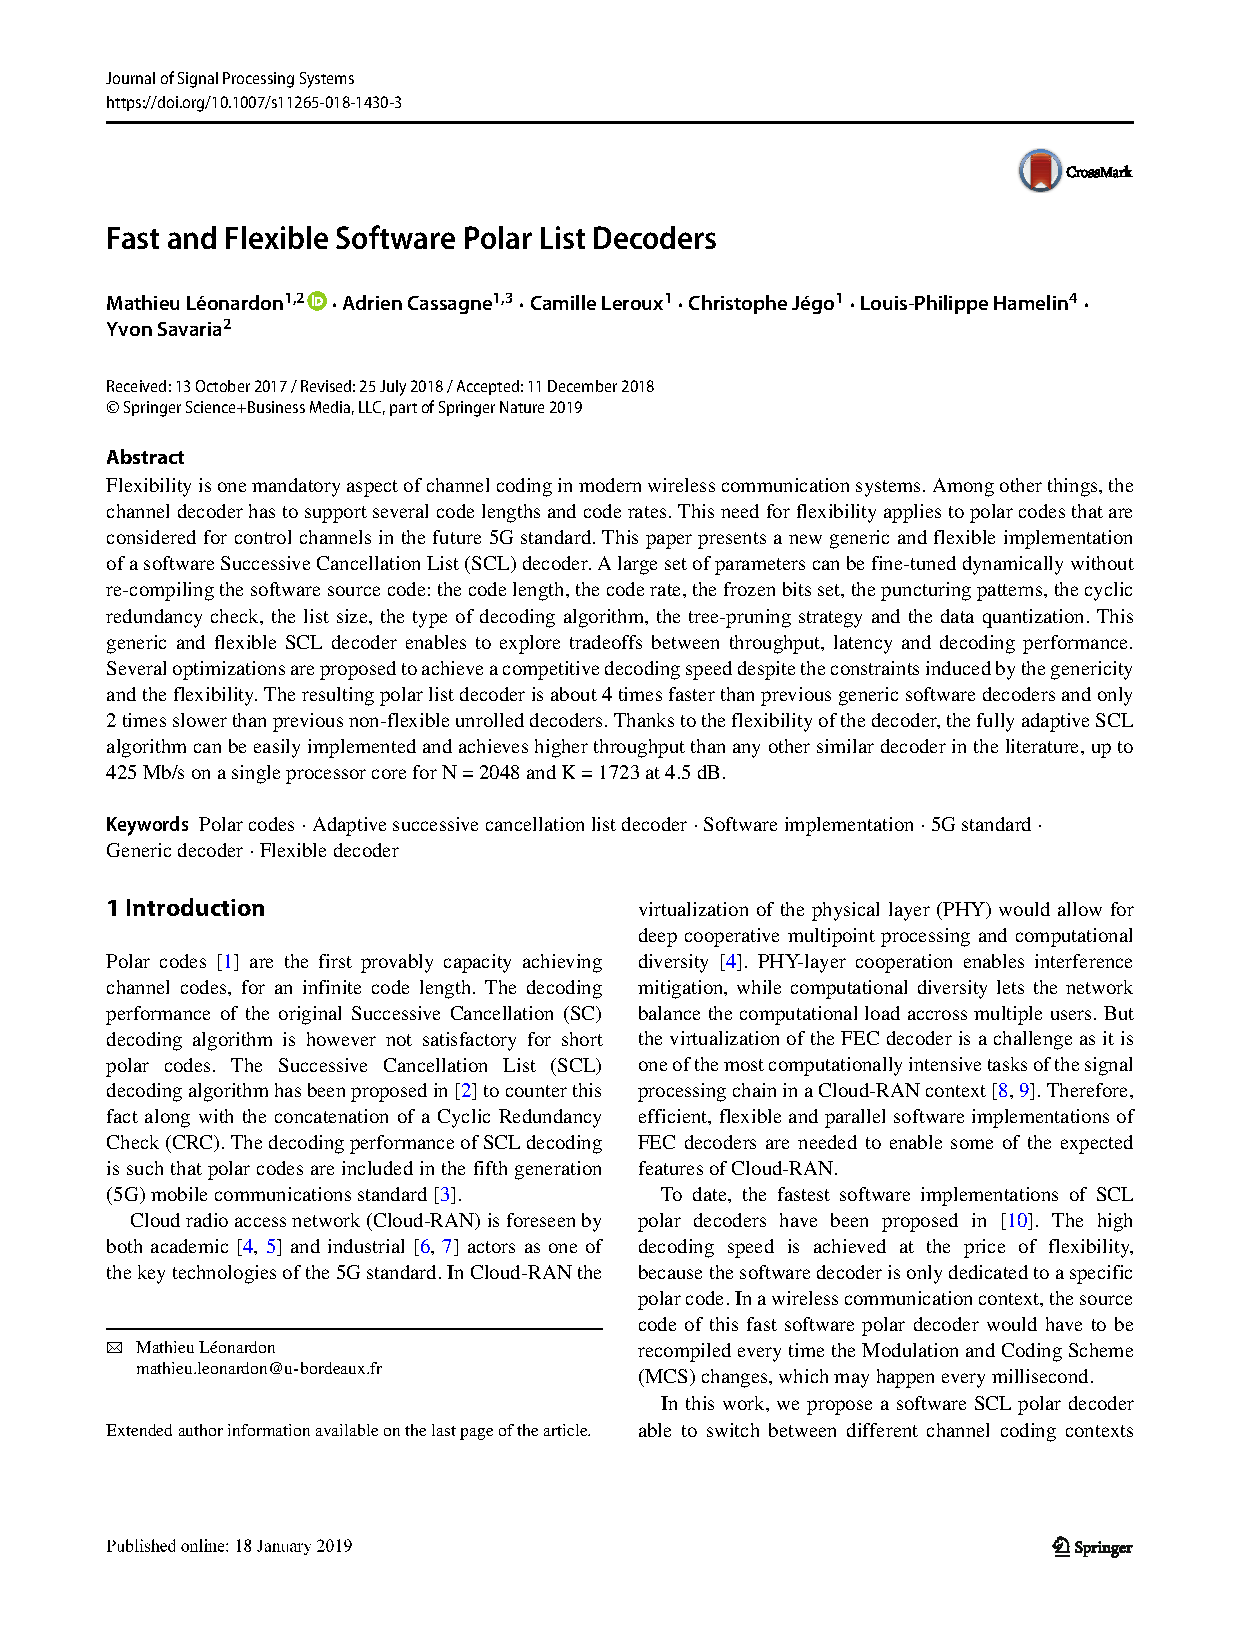
\includepdf[pages=1,pagecommand={\section{Articles}\vspace{1cm}\subsection{Fast and Flexible Software Polar List Decoders}},width=\paperwidth, offset=80 -160]{pieces/article_fast_list.pdf}
\includepdf[pages=2-,pagecommand={},width=\paperwidth, offset=80 -40]{pieces/article_fast_list.pdf}

\includepdf[pages=1,pagecommand={\subsection{Custom Low Power Processors for Polar Decoding}},width=\paperwidth, offset=80 -100]{pieces/article_custom.pdf}
\includepdf[pages=2-,pagecommand={},width=\paperwidth, offset=80 -40]{pieces/article_custom.pdf}

\includepdf[pages=1,pagecommand={\subsection{Transport Triggered Polar Decoders}},width=\paperwidth, offset=80 -140]{pieces/article_ttpd.pdf}
\includepdf[pages=2-,pagecommand={},width=\paperwidth, offset=80 -40]{pieces/article_ttpd.pdf}


% Rapport de soutenance
\includepdf[pages=1,pagecommand={\section{Rapports de th�se}\vspace{1cm}\subsection{Rapport de soutenance}},width=\textwidth, offset=80 -100]{pieces/rapport_soutenance.pdf}
\includepdf[pages=2-,pagecommand={},width=\textwidth, offset=80 -40]{pieces/rapport_soutenance.pdf}

% Rapport Amer
\includepdf[pages=1,pagecommand={\subsection{Rapport - Amer Baghdadi}},width=\textwidth, offset=80 -100]{pieces/rapport_amer_baghdadi.pdf}
\includepdf[pages=2-,pagecommand={},width=\textwidth, offset=80 -40]{pieces/rapport_amer_baghdadi.pdf}

% Rapport Emmanuel
\includepdf[pages=1,pagecommand={\subsection{Rapport - Emmanuel Casseau}},width=\textwidth, offset=80 -100]{pieces/rapport_emmanuel_casseau.pdf}
\includepdf[pages=2-,pagecommand={},width=\textwidth, offset=80 -40]{pieces/rapport_emmanuel_casseau.pdf}



\section{Pi�ce d'identit�}
\vspace*{2.7cm}
\begin{center}
\includegraphics{pieces/passeport.jpg}
\end{center}

\newpage
\includepdf[pages=-,pagecommand={\section{Dipl\^ome de Doctorat}},width=\textwidth, offset=80 -80]{pieces/Diplome.pdf}

\end{document}
